\chapter{Manuales}


\section{Manual de usuario}
\bigskip

El cliente o usuario tendrá una primera impresión de la \textit{portada} del servicio web. Simplemente se le mostrará el logo y título del servicio y podrá avanzar hacia las funcionalidades mediante un botón, o haciendo \textit{scroll} hacia abajo.

\bigskip
\begin{figure}[h]
	\centering
	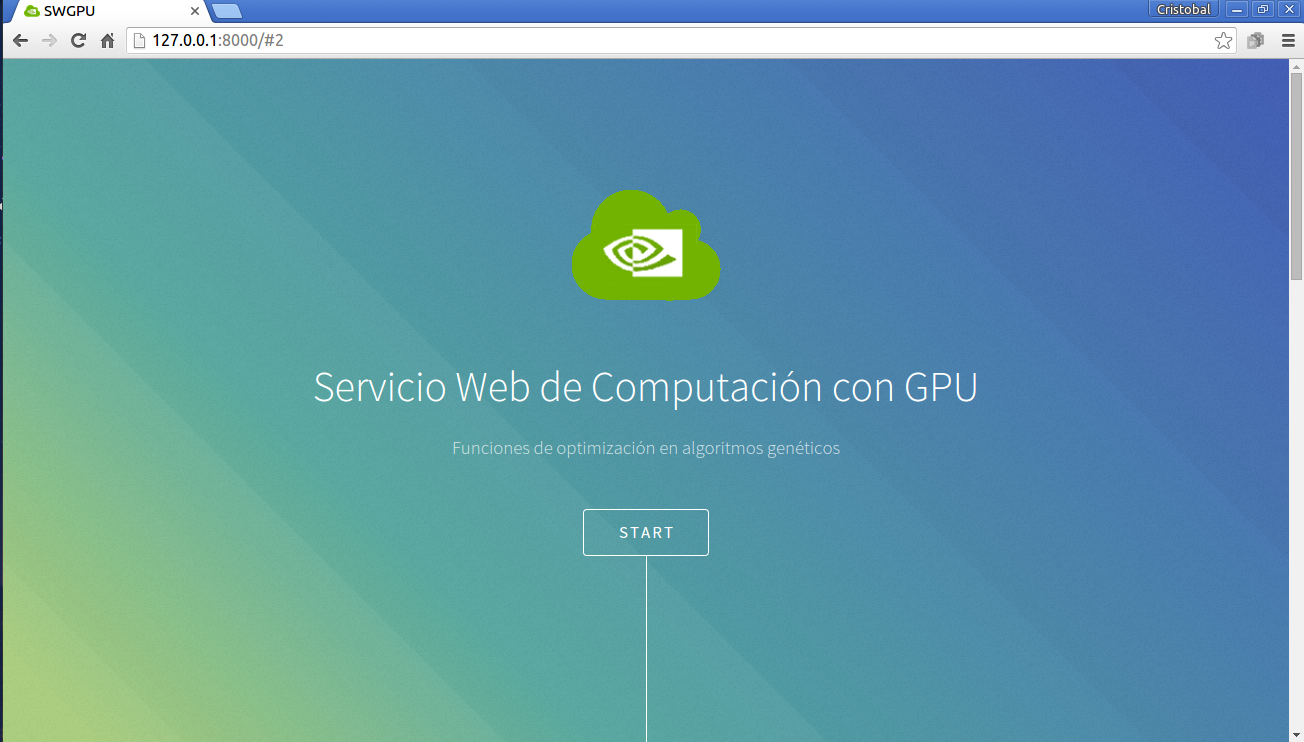
\includegraphics[width=1\linewidth]{../images/captura_web_1}
	\caption[Captura de la portada del servicio web]{Captura de la portada del servicio web}
	\label{fig:captura_web_1}
\end{figure}


Una vez avance podrá ver los servicios disponibles: ejecutar un algoritmo genético y que se optimizado mediante la función de Ackley o de Rastrigin. Para acceder a dichos servicios sólo tendrá que \textit{clickar} sobre el servicio que quiera y se desplegará.

\bigskip
\begin{figure}[h]
	\centering
	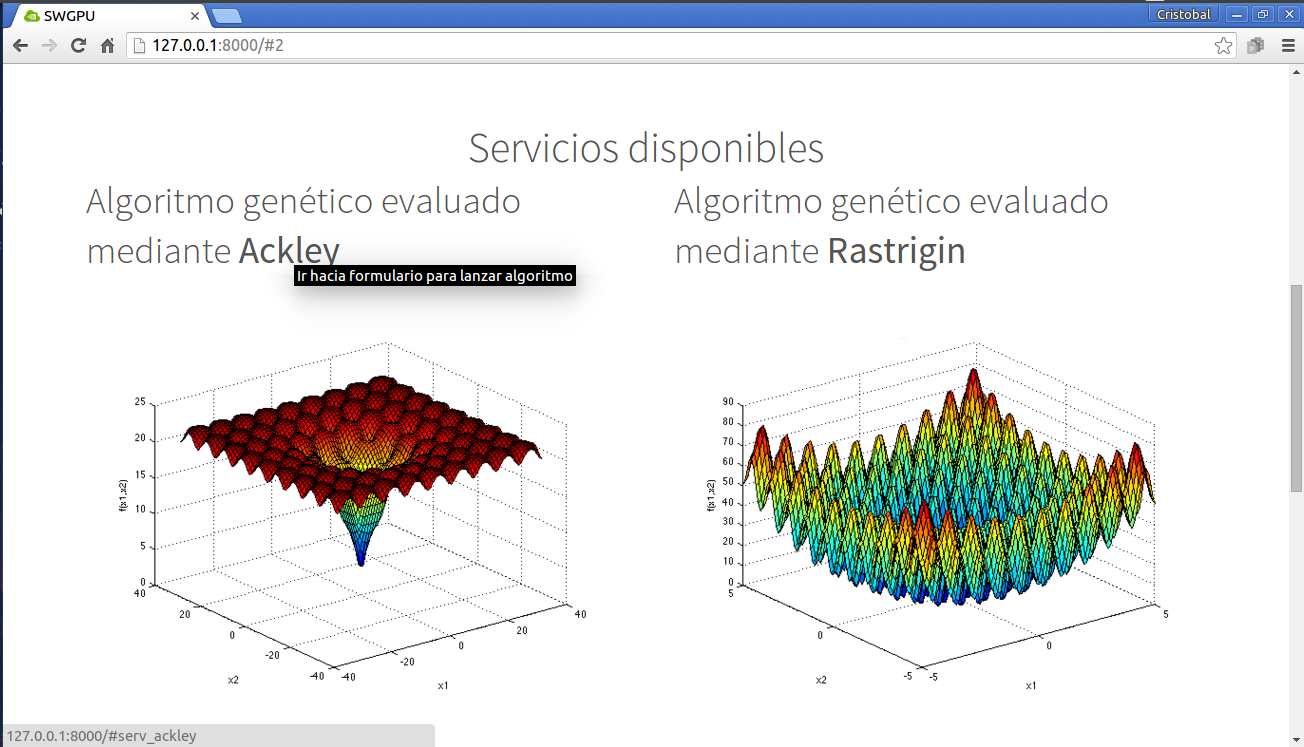
\includegraphics[width=0.9\linewidth]{../images/captura_web_2}
	\caption[Captura de los servicios disponibles]{Captura de los servicios disponibles}
	\label{fig:captura_web_2}
\end{figure}


\bigskip
Una vez elegido el servicio se desplegará su correspondiente formulario. Para acceder a él el usuario sólo tendrá que \textit{clickar} sobre el título en la pantalla de \textit{Servicios disponibles} o avanzar hacia el mediante \textit{scroll}. Una vez en el formulario se le mostrarán los valores por defecto de cada parámetro, pudiendo cambiar cada uno de manera sencilla:

\bigskip
\begin{figure}[h]
	\centering
	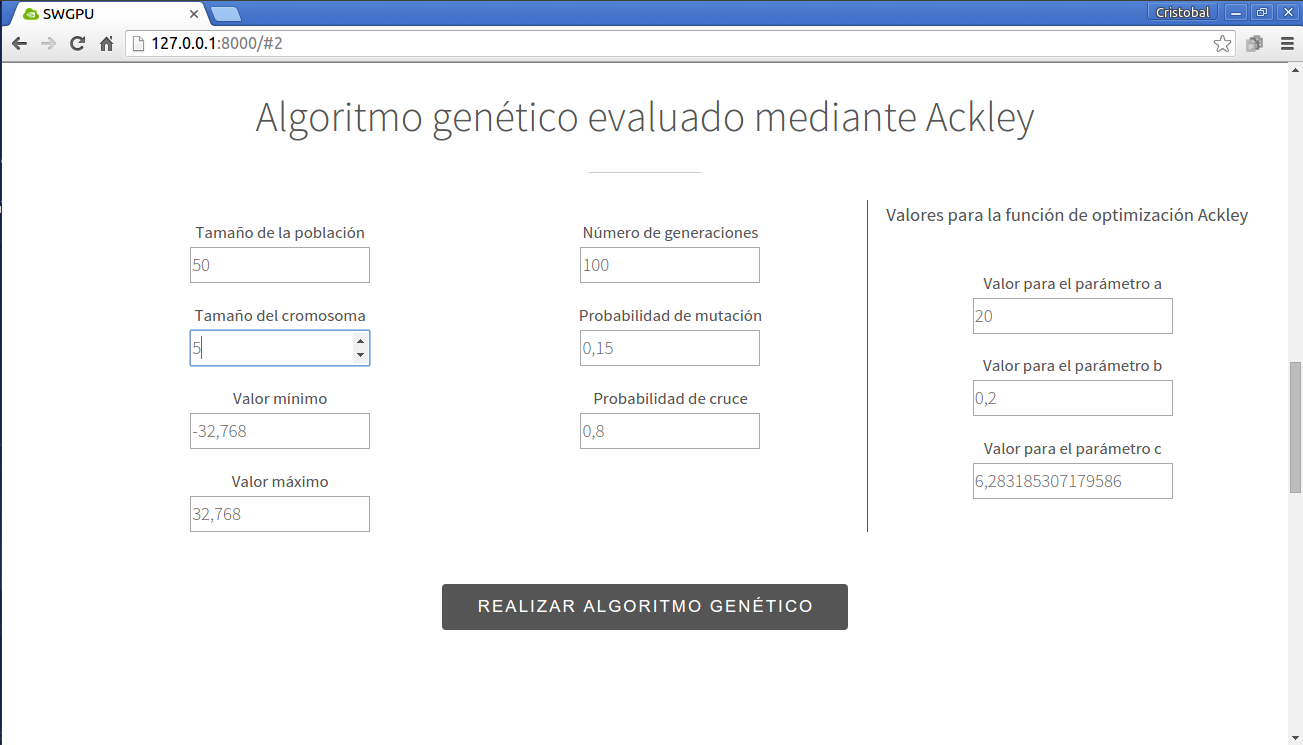
\includegraphics[width=0.9\linewidth]{../images/captura_web_3}
	\caption[Formulario para lanzar el algoritmo genético]{Formulario para lanzar el algoritmo genético}
	\label{fig:captura_web_3}
\end{figure}

\bigskip
También se asegurará que se introducen los valores correctamente:

\bigskip
\begin{figure}[h]
	\centering
	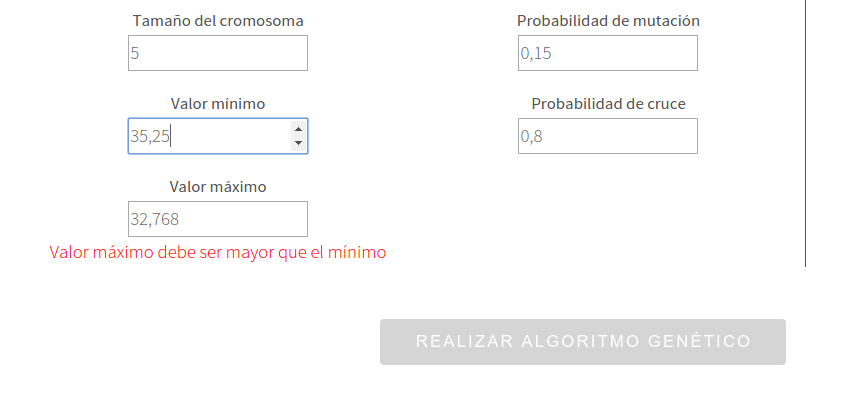
\includegraphics[width=0.7\linewidth]{../images/captura_web_3_1}
	\caption[Mensaje de error en el formulario]{Mensaje de error en el formulario}
	\label{fig:captura_web_3_1}
\end{figure}


\bigskip
Y una vez realizado el algoritmo genético, ya se podrá acceder a los resultados. Para ello sólo hay que avanzar hacia abajo o mediante el botón de V\textit{er resultados}. Se mostrará información sobre la petición (hora y parámetros), datos sobre el cómputo (dispositivo usado o tiempo invertido) y los resultados obtenidos.

\bigskip
\begin{figure}[h]
	\centering
	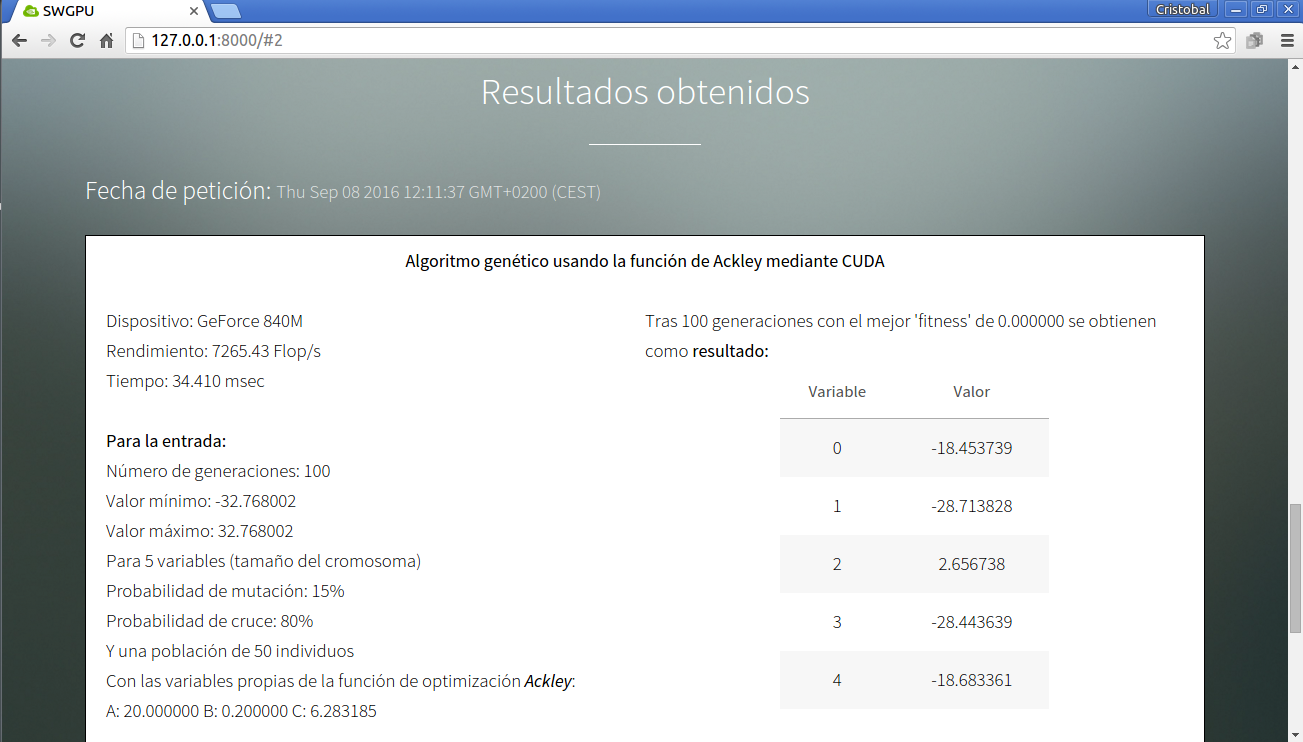
\includegraphics[width=1\linewidth]{../images/captura_web_4}
	\caption[Resultados obtenidos]{Resultados obtenidos}
	\label{fig:captura_web_4}
\end{figure}


\newpage
\bigskip
Por último, se muestra al final, aunque se puede acceder siempre a él, una sección de contacto. Se podrá poner en contacto con el administrador del sistema.

\bigskip
\begin{figure}[h]
	\centering
	
\includegraphics[width=0.9\linewidth]{../images/captura_web_5}
	\caption[ ]{ }
	\label{fig:captura_web_5}
\end{figure}


\bigskip
Además, como añadido, se facilita la ayuda sobre parámetros y ejecución del ejecutable \textit{geneticAlgorithm} como parte independiente, sin requerir del servicio web, como se puede ver en la Figura \ref{fig:peticion_ejecutable} del capitulo anterior.


\newpage
\section{Manual de despliegue}
\bigskip

A continuación se explicará la forma y requisitos de despliegue del sistema. 

\subsection{Requisitos para el despliegue}
\bigskip

Para el correcto despliegue de la aplicación habrá que contar con sus 2 partes: el servicio web y el procesamiento con GPU mediante CUDA.

\bigskip
Para lanzar el servicio web:
\begin{itemize}
	\item Apache (versión 2.4 o superior)
	\item Python (Python 2)
	\item Django  (versión 1.10 o superior)
\end{itemize} 

\bigskip
Y para el procesamiento mediante CUDA:
\begin{itemize}
	\item Dispositivo NVIDIA
	\item Drivers NVIDIA (versión 352.xx)
	\item CUDA 7.5
	\item C++ (versión 4.x)
\end{itemize} 

\subsection{Despliegue}
\bigskip


Una vez que se cumplen los requisitos, sólo habrá que lanzar el servicio web, ya que el procesamiento usando la GPU se gestiona sólo mediante el ejecutable \textit{geneticAlgorithm}.

Para ello el servidor Apache tendrá que estar activo (se puede activar ejecutando \textit{service apache2 restart}) y lanzar el proyecto Django con el proyecto: dentro del directorio SWGPU ejecutar, junto con la URL donde lanzar el sistema \textit{python manage.py runserver [URL]}


\subsection{Despliegue automatizado}
\bigskip
También se proporcionará el script o archivo \textit{despliegue.sh} para automatizar la tarea de despliegue.

Simplemente habrá que ejecutarlo (dentro del \textit{directorio SWGPU},mediante la orden \textbf{sudo ./despliegue.sh}) y luego especificar la URL donde se desplegará. El script comprobará los requisitos antes citados, preparará el servidor y lanzará el sistema.

En la siguiente captura se ve como se lanza el servidor:

\bigskip
\begin{figure}[h]
	\centering
	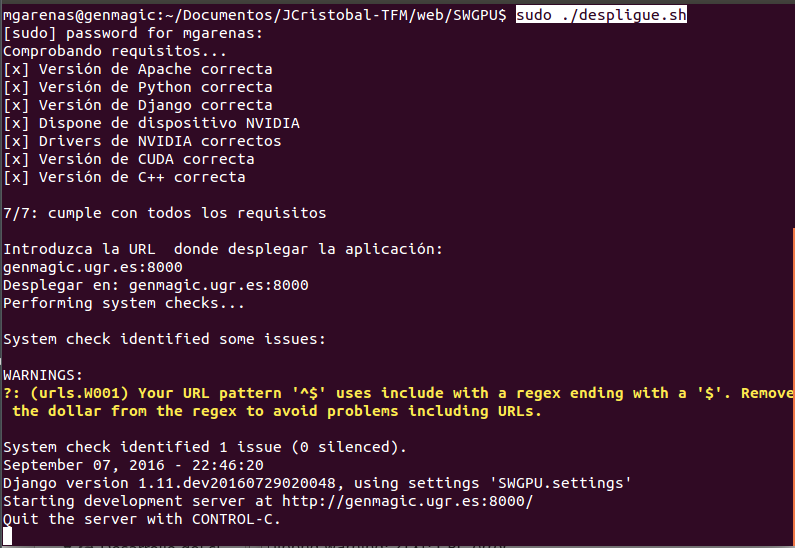
\includegraphics[width=1\linewidth]{../images/prueba_despliegue}
	\caption[Captura del despliegue automático]{Captura del despliegue automático}
	\label{fig:prueba_despliegue}
\end{figure}


